%%%%%%%%%%%%%%%%%%%%%%%%%%%%%%%%%%%%%%%%%%%%%%%%%%%%%%%%%%%%%%%%%%%%%
\documentclass{ifacconf}
%\documentclass[letterpaper,10pt,conference]{ieeeconf}  
% Comment the above line out if you need a4paper, and use instead:
%\documentclass[a4paper, 10pt, conference]{ieeeconf}      
%\IEEEoverridecommandlockouts  % This command is only needed if 
%                              % you want to use the \thanks command.
%\overrideIEEEmargins          % Needed to meet printer requirements.
\usepackage{amsmath,amssymb}
\usepackage{graphicx,epsfig,natbib}
%\usepackage{mathptmx,times} % if new font selection scheme installed
%\usepackage{mathtools}
%\usepackage{mathrsfs}
%\usepackage{url}
%\usepackage{epsfig} % for postscript graphics files
%%%%%%%%%%**********%%%%%%%%%%**********%%%%%%%%%%**********%%%%%%%%%%
\newtheorem{theorem}{Theorem}[section]
\newtheorem{corollary}[theorem]{Corollary}
\newtheorem{lemma}[theorem]{Lemma}

\newtheorem{proposition}[theorem]{Proposition}
%\newtheorem{definition}[theorem]{Definition}
%\newtheorem{example}[theorem]{Example}
%\newtheorem{problem_statement}[theorem]{Problem Statement}
%\newtheorem{remark}[theorem]{Remark}

\newcommand{\BE}{\begin{equation}}
\newcommand{\BEQ}[1]{\BE\label{#1}} % Changed by Olof
\newcommand{\EEQ}{\end{equation}}
\newcommand{\rfb}[1]{\mbox{\rm
   (\ref{#1})}\ifx\undefined\stillediting\else:\fbox{$#1$}\fi}
\newenvironment{matr}[1]{\left[ \begin{array}{#1}}{\end{array}
                         \right]}
\renewcommand{\cline}{{\mathbb C}}
\newcommand{\rline}  {{\mathbb R}}
\renewcommand{\l}    {{\lambda}}
\renewcommand{\L}    {{\Lambda}}
\renewcommand{\o}    {{\omega}}
\renewcommand{\e}    {{\varepsilon}}
\renewcommand{\half} {{\frac{1}{2}}}
\newcommand{\m}      {{\hbox{\hskip 1pt}}}
\newcommand{\nm}     {{\hbox{\hskip -3pt}}}
\newcommand{\dd}     {{\rm d\hbox{\hskip 0.5pt}}}
\newcommand{\Amscr}  {{\mathcal{A}}}
\newcommand{\Bmscr}  {{\mathcal{B}}}
\newcommand{\Cmscr}  {{\mathcal{C}}}
\newcommand{\Emscr}  {{\mathcal{E}}}
\newcommand{\Kmscr}  {{\mathcal{K}}}
\newcommand{\Mmscr}  {{\mathcal{M}}}
\newcommand{\Nmscr}  {{\mathcal{N}}}
\newcommand{\Xmscr}  {{\mathcal{X}}}
\newcommand{\FORALL} {{\hbox{$\hskip 11mm \forall \;$}}}
\newcommand{\rarrow} {{\rightarrow}}

%\makeatother
% See the \addtolength command later in the file to balance the 
% column lengths on the last page of the document

\begin{document}
\begin{frontmatter}

%%%%%%%%%%**********%%%%%%%%%%**********%%%%%%%%%%**********%%%%%%%%%%
\title{Stability analysis for two coupled synchronous generators}
\author[First]{Elad Venezian}
\author[Second]{George Weiss}

\address[First]{School of EE, Tel Aviv University Ramat Aviv 69978, 
        Israel \\ (e-mail: eladv@gmail.com)}
\address[Second]{School of EE, Tel Aviv University Ramat Aviv 69978, 
        Israel \\ (e-mail: gweiss@eng.tau.ac.il)}

\begin{abstract}
We investigate the stability of a microgrid composed of two identical
synchronous generators, inductive lines and resistive loads, without
using any model reduction for ``fast'' variables. We derive sufficient
conditions for local exponential stability, with a region of
attraction that includes any initial state such that the states of the
generators are sufficiently close to each other. This implies that if
by some control technique we can bring the angular velocities close
enough, regardless how far the system is from the equilibrium state,
then the generators will synchronize.
\end{abstract}

\begin{keyword}
synchronous generator, microgrid, synchronization, local stability, 
invariant manifold, region of attraction. 
\end{keyword}

\end{frontmatter}

%%%%%%%%%%**********%%%%%%%%%%**********%%%%%%%%%%**********%%%%%%%%%%
\section{Introduction}

The grid is an enormously complex nonlinear and randomly varying 
system for which rigorous stability analysis is impossible. 
Many techniques and models that have been developed to assess the 
stability of a power grid, using simplifying assumptions and reduced
models, see for instance \cite{Kundur}, \cite{GrSt2014}, 
\cite{SauerPai1998}, \cite{GOBS:03}, \cite{DoBull:12}.

In recent years, due to the increasing penetration of renewable energy
resources, which connect to the grid via power converters and produce
an intermittent power output, it is not clear whether the traditional
models and methods for controlling the power grid will succeed to
control it. Therefore, there is an increasing interest in the
fundamental mathematical models and stability analysis for the grid,
see for instance \cite{DoBull:12}, \cite{PoDoBu:13}, \cite{CaTa:14},
\cite{NaWe:14}, \cite{NaWe:15}, \cite{DePersiSchaft:16}.

An important concept that facilitate the integration of the renewable
energy resources into the electricity grid is the microgrid concept
\cite{GreenProdanovic:07,Schiffer_2016_survey}. A microgrid can work 
as an independent isolated network (islanded mode), or alternatively
in grid connected mode it behaves as a single controllable generator 
or load from the viewpoint of the remaining electrical system.
In islanded mode, the frequency, voltage and power sharing are 
actively controlled within the microgrid. Controlling the frequency 
and voltage and balance the active/reactive load demand, is one of 
the main challenges of the microgrid system 
\cite{Shafiee_2016,Zhong:13}.

The {\em synchronous generator} (SG) is the main power source of the
electricity grid. The mathematical model of a SG (see the earlier
references and in addition \cite{Walker:94}, \cite{Fitzgerald:03},
\cite{MaWe:15}, etc.) is complex and difficult to use as a component
when we model a large network. Stability analysis is usually done
either by simulation, or analytically on simplified models, in which
the SGs are connected in a simple network and each SG is represented
by reduced order equations, see for instance \cite{DoBull:12} and
\cite{PoDoBu:13}. The reduced model of a SG is often obtained by
treating the stator currents as fast variables, thus eliminating them
from the state variables via the singular perturbation approach (see,
for instance, \cite{Khalil}) and keeping only the rotor angle, the
rotor angular velocity and the rotor field as relevant state
variables, see for instance \cite{Kundur} and \cite{SauerPai1998}.

It is desirable to know if for a given grid which contains SGs and a
loads, the SGs tend to synchronize (for initial states in a reasonably
large region) and if yes, if the grid frequency and power flows
remains stable. 

Here we study a microgrid composed of a two identical SGs connected to
a resistive load, as shown in Figure \ref{fig:TICSGThreePhase}. These
generators are driven by identical prime movers, that have frequency
droop control. Our main result is that if the difference between the
initial states of the SGs is sufficiently small, then the state of the
entire system converges at an exponential rate to a unique stable
equilibrium point in the state space $\Xmscr$, a 7-dimensional
manifold. In $\Xmscr$, the angle difference $\delta$ between the
generators is counted modulo $2\pi$. In some arguments we use
$\rline^7$ as a state space, and then $\delta$ can take any real
value.

%%%%%%%%%%**********%%%%%%%%%%**********%%%%%%%%%%**********%%%%%%%%%%
\begin{figure} % Figure 1: tree phase TICSG system
\centering 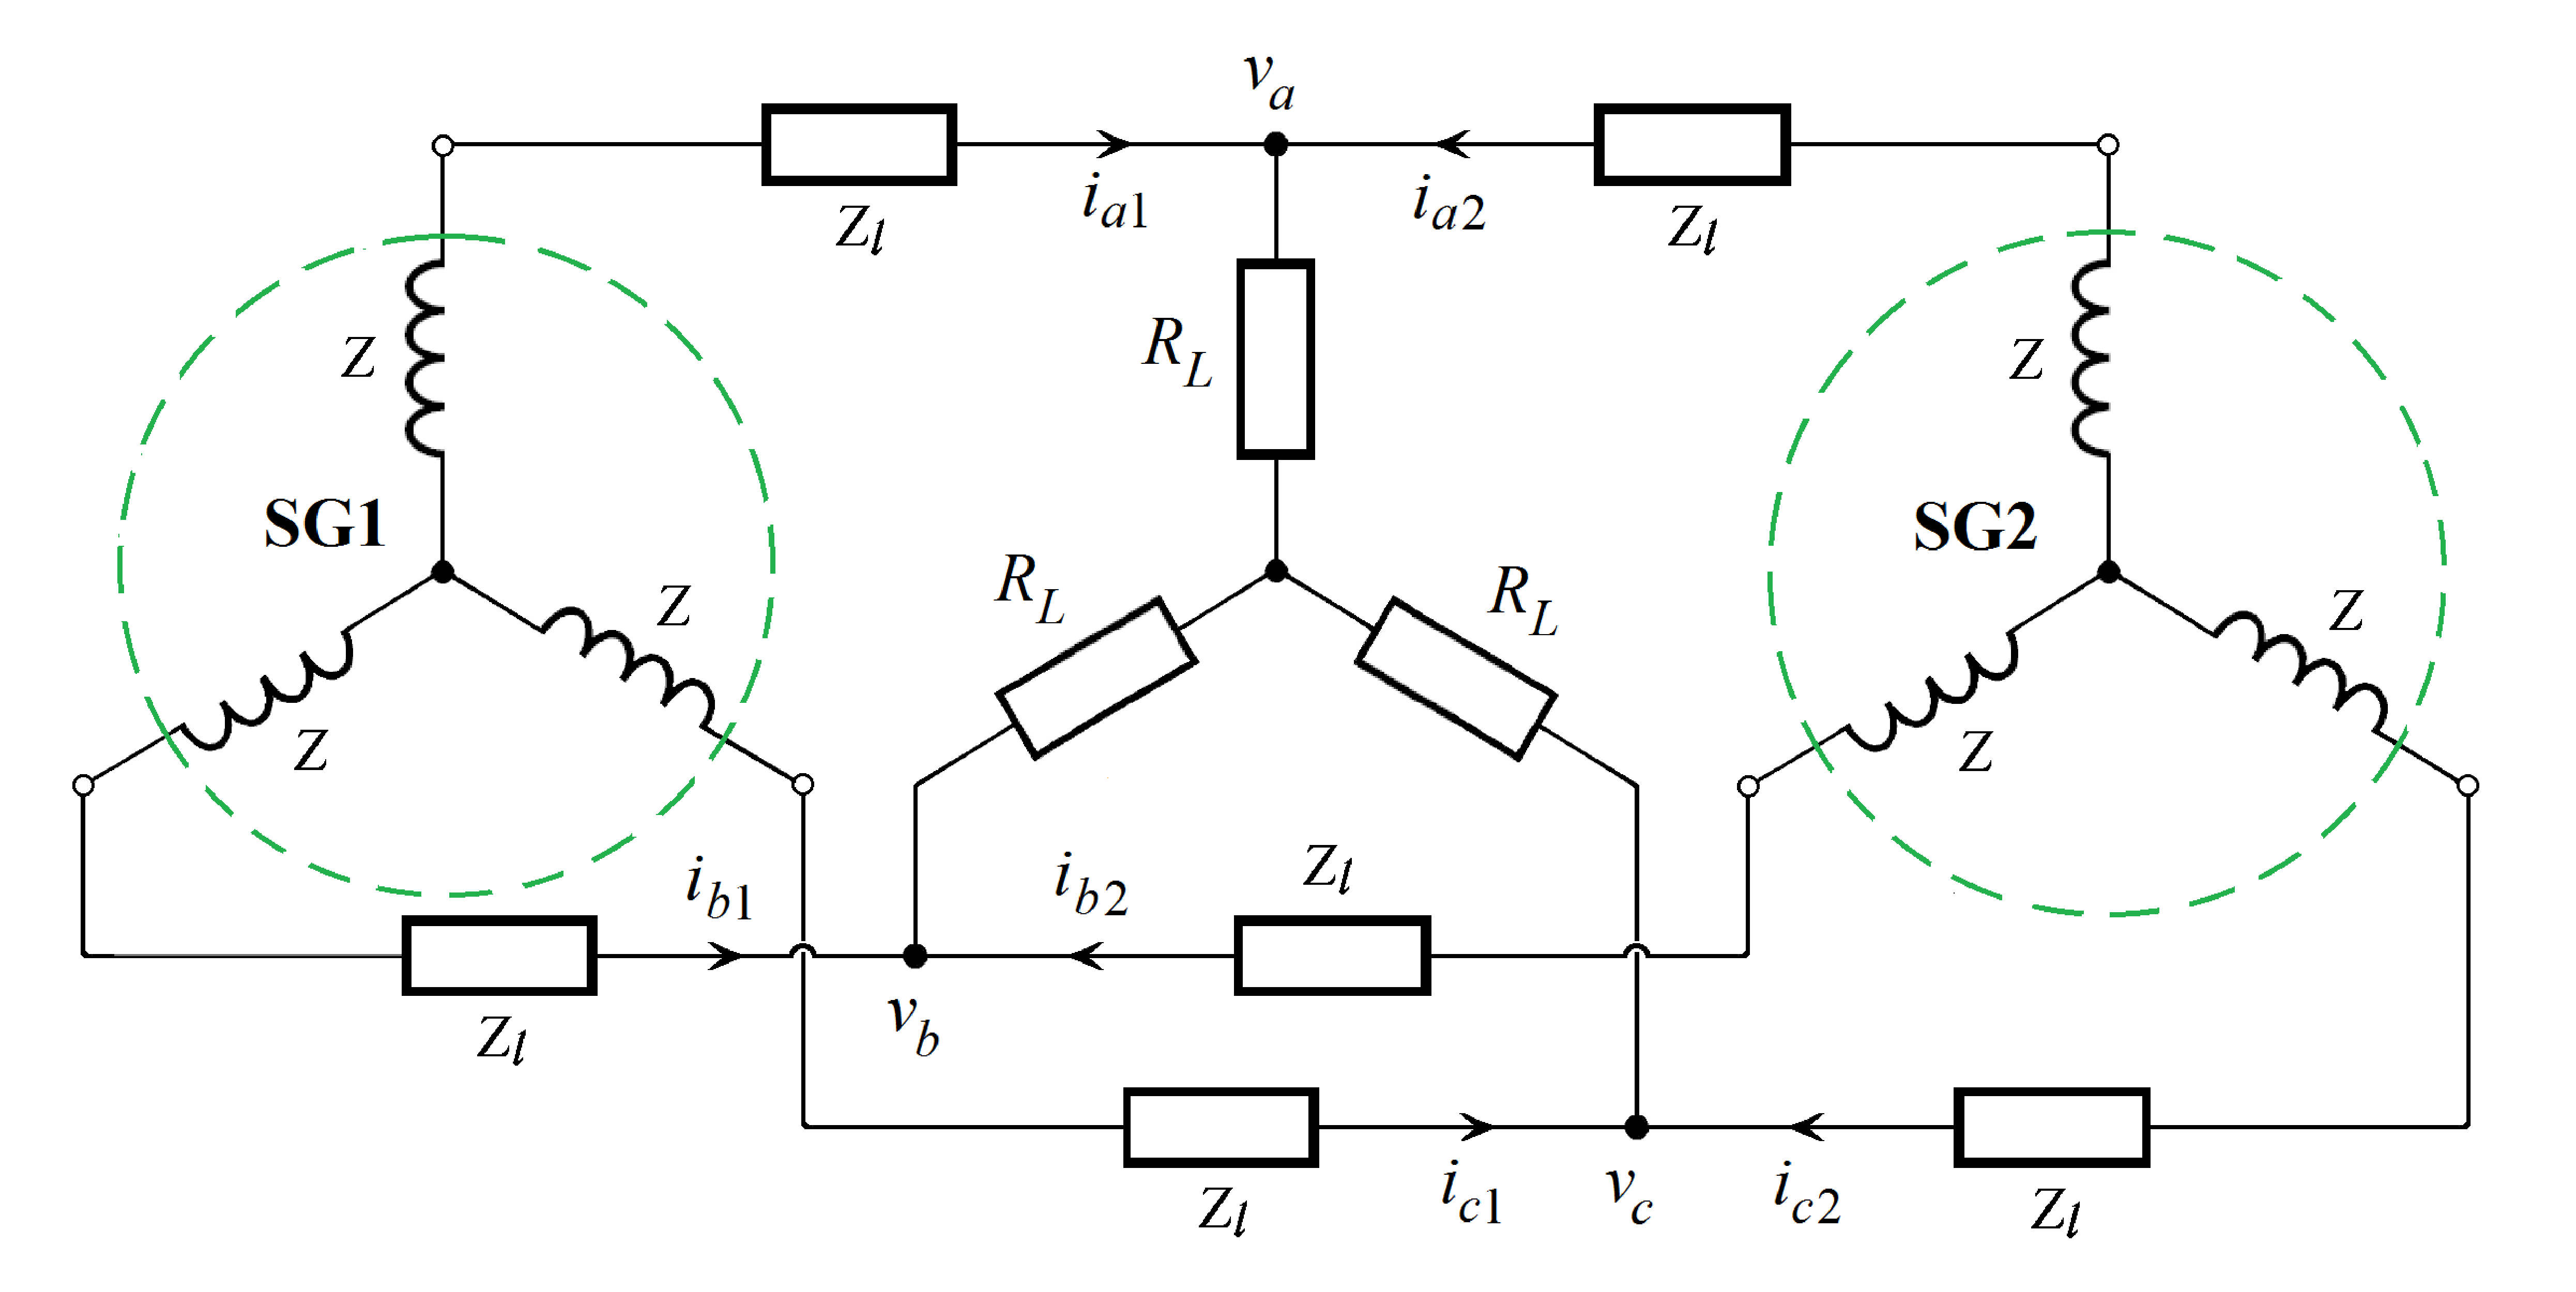
\includegraphics[width=8.5cm]{full_circuit_with_2_SGs}
\caption{The two identical coupled SGs (TICSG) model, showing the 
stator windings, the line impedances $Z_l$ and the load resistors 
$R_L$, but not showing the rotor windings or the prime movers.}
\label{fig:TICSGThreePhase}
\end{figure}
%%%%%%%%%%**********%%%%%%%%%%**********%%%%%%%%%%**********%%%%%%%%%%

We illustrate our results by simulations. In particular, we show an
example of two SGs where the region of attraction of the stable
equilibrium point contains the submanifold where the generators have
equal states (as it always does), but it does not contain all
$\Xmscr$.

%%%%%%%%%%**********%%%%%%%%%%**********%%%%%%%%%%**********%%%%%%%%%%
\section{Modeling a single SG} \label{sec2} % Section 2

We recall the equations for a SG connected to an exernal voltage and
having a constant field (or rotor) current $i_f$, following the
notation in \cite{ZhWe:11}, see also \cite{NaWe:14,NaWe:15},
\cite{VeWe:16}.

The rotor of a SG is a coil on a magnetic core that spins inside a
circular cavity in the stator, having the angle $\theta$ with respect
to a reference angle. We consider that there is no neutral
connection and no damper windings. The stator windings can be regarded
as connected coils with self inductance $L$, mutual inductance $-M$,
and resistance $R_s$ (the parameters $L_f,R_f,L,M,R_s$ are
positive). We assume no magnetic saturation effects in the iron core
and no Eddy currents. The stator terminals are labeled with the
letters $a,b,c$ and the vector of voltages on the stator terminals is
denoted by $v=\left[v_a\ v_b\ v_c\right]^\top$. 

The mutual inductance between the rotor coil and each of the stator
coils is a sinusoidal function of $\theta$, with amplitude $M_f>0$.
In order to represent the voltages and currents in a more convenient 
way, we apply the Park transformation with respect to the rotor 
angle, obtaining the voltages $v_d,v_q,v_0$ and the currents $i_d$, 
$i_q$, $i_0$. We denote \vspace{-1mm}
$$\o \m=\m \dot{\theta} \m,\qquad m=\sqrt{\frac{3}{2}}M_{f}.$$ 
As shown in the sources cited at the beginning of this section, we 
obtain the following model for a SG:
\BEQ{eq:SingleSGDynamics}
   \frac{\dd}{\dd t}\nm\left[\nm\begin{array}{c} L_s i_d\\ L_s i_q\\ 
   J\o\end{array} \right] = \left[\nm \begin{array}{ccc} -R_s & 
   \o L_s & 0\\ -\o L_s & -R_s & -mi_f\\ 0 & mi_f & -D_p \end{array}
   \nm\right] \nm \left[\begin{array}{c} i_d\\ i_q\\ \o 
   \end{array} \right] + \left[\nm \begin{array}{c} -v_d\\ -v_q
   \\ T_m \end{array} \nm\right],
\end{equation}
where $J$ is the moment of inertia of the rotor, $T_m-D_p\o$ is is the
torque coming from the prime mover, $D_p$ is a the frequency droop
coefficient employed in the prime movers connected to the
generators. If any viscous friction is present, it can be absorbed
into the term $D_p\o$. The parameters $J,T_m,D_p$ are positive.  The
feedback term $D_p\o$ is used to control the frequency of the grid,
see \cite{Kundur}, \cite{PoDoBu:13}, \cite{CaTa:14}, \cite{ZhWe:11}.

%%%%%%%%%%**********%%%%%%%%%%**********%%%%%%%%%%**********%%%%%%%%%%
\section{TICSG modeling} \label{sec3} % Section 3

In this section we develop the TICSG model that represent two 
identical SGs connected to a common resistive load, as shown in
Figure \ref{fig:TICSGThreePhase}, assuming constant field currents.
The model of each SG is as in Section \ref{sec2}.

We denote the SG rotor angles by $\theta_1$ and $\theta_2$ and
$\o_1=\dot\theta_1$, $\o_2=\dot\theta_2$. We assume that identical
prime movers act on the generators, producing the torques
$T_{m}-D_p\o_i$, $i\in\{1,2\}$. By symmetry, we assume that the
voltages at the (non-connected) midpoints of the generators and the
load are zero. We denoted the phase voltages on the load by
$v=\left[v_a\ v_b\ v_c \right]^\top$, the currents of the first
generator by $i_1=\left[i_{a1} \ i_{b1}\ i_{c1}\right]^\top$ and 
similarly for the currents of the second generator.
%by $i_2=\left[i_{a2}\ i_{b2}\ i_{c2}\right]^\top$.

In Figure \ref{fig:TICSGThreePhase} we have indicated by $Z$ the
equivalent impedance of each SG stator, $Z=sL_s+R_s$. The line that
connects the SG to the load has its impedance $Z_l$ that can be
modeled as a resistance and an inductance in series, but these values
can simply be added to the parameters $R_s$ and $L_s$ of the SG. After
this simplification, each phase of the circuit from Figure
\ref{fig:TICSGThreePhase} is as in Figure \ref{fig:TICSGOnePhase}.

%%%%%%%%%%**********%%%%%%%%%%**********%%%%%%%%%%**********%%%%%%%%%%
\begin{figure} % Figure 3: Tree phase TICSG system
\centering 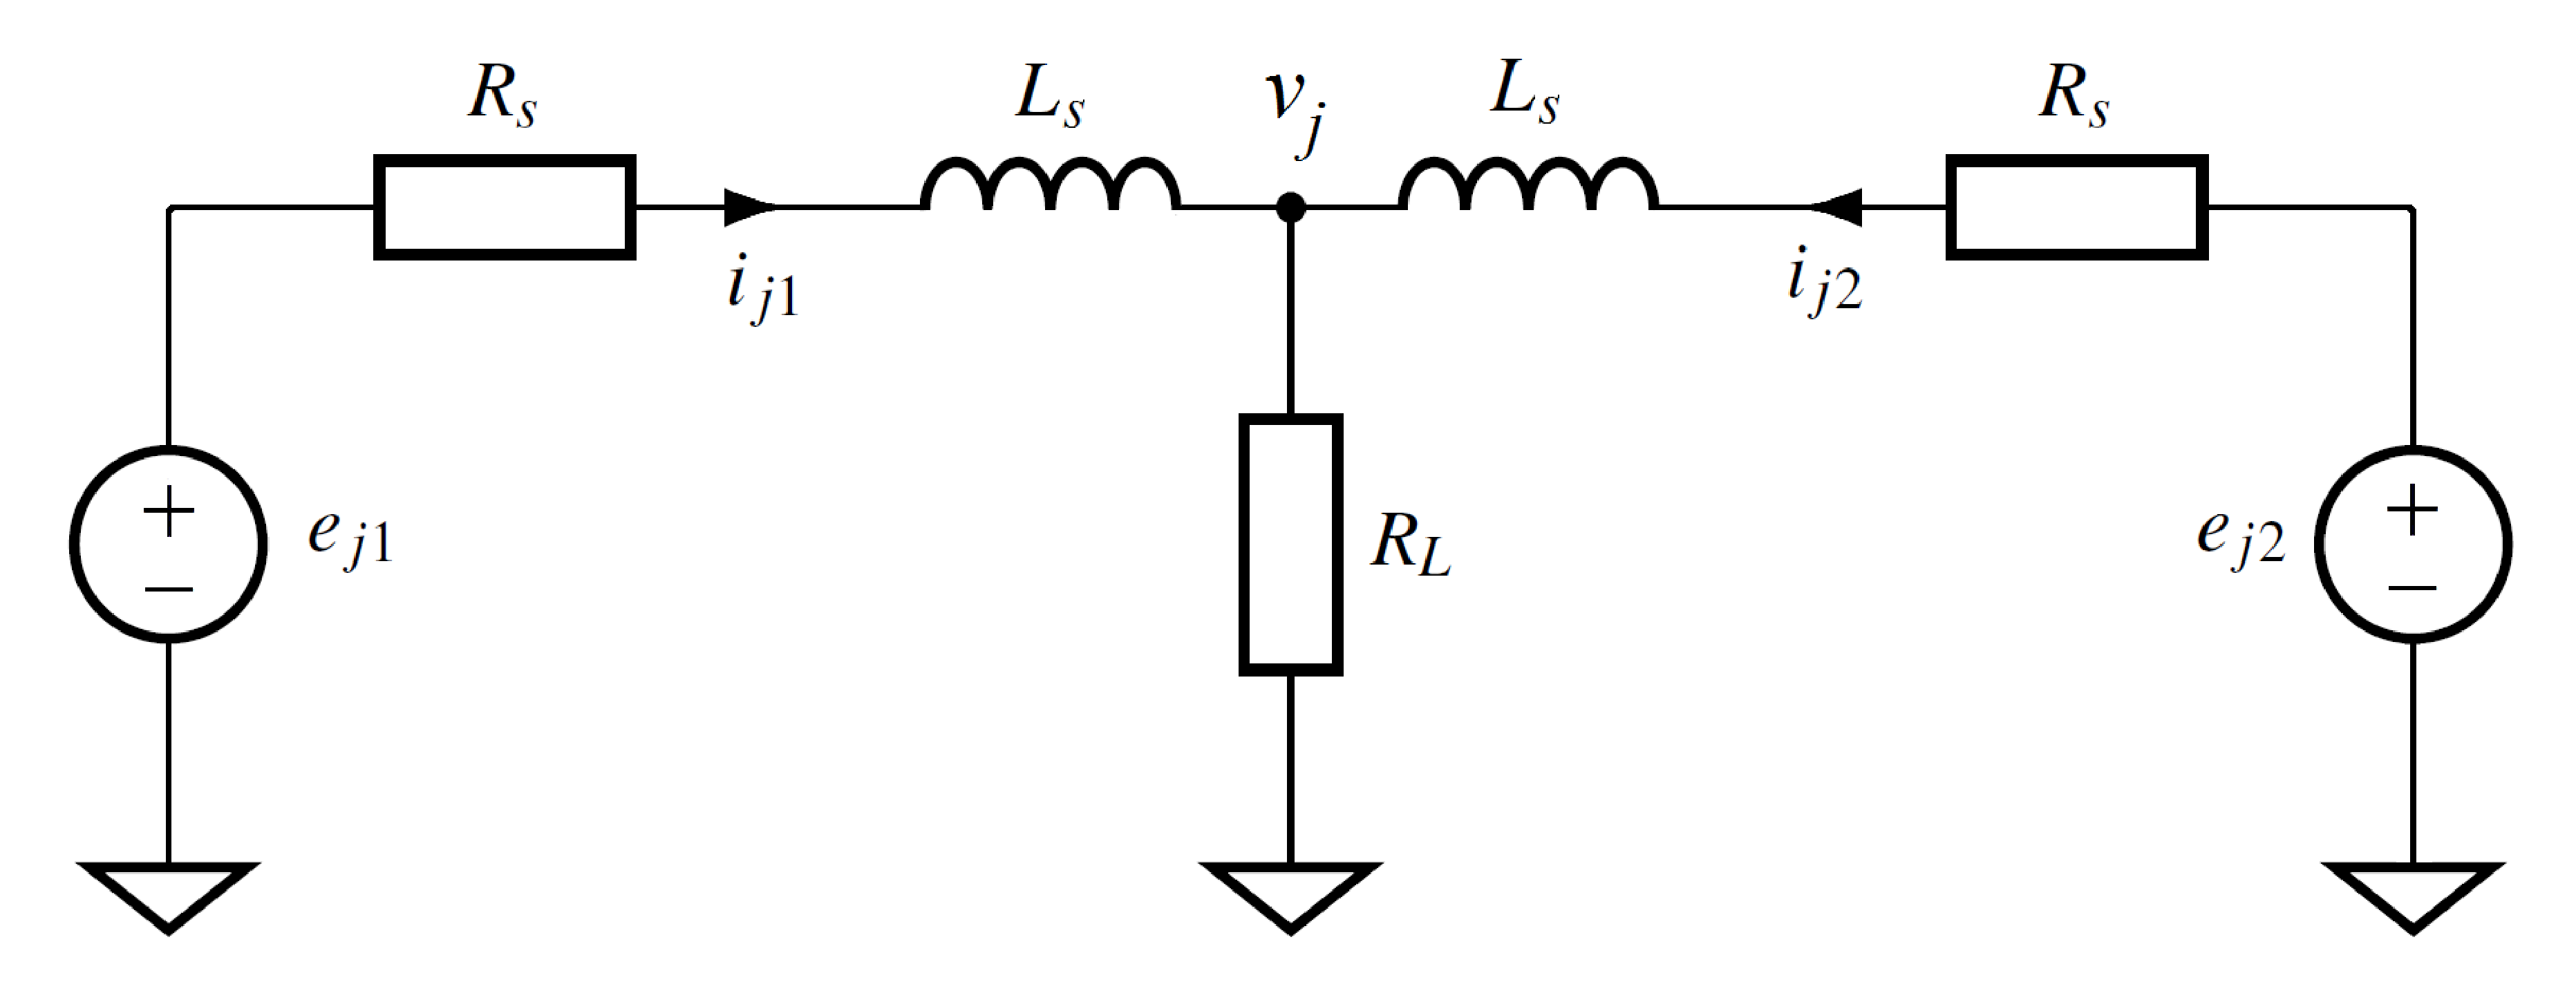
\includegraphics[width=8cm]{one_phase.eps}
\vspace{-3mm}
\caption{The TICSG model - equivalent circuit for one phase, 
$j\in\{a,b,c\}.$} \label{fig:TICSGOnePhase}
\end{figure}
%%%%%%%%%%**********%%%%%%%%%%**********%%%%%%%%%%**********%%%%%%%%%%

In order to use the model \eqref{eq:SingleSGDynamics} for each SG, we
apply the Park transformation (defined in the previous section) to the
load voltages, $\left[ v_{d1}\ v_{q1}\ v_{01}\right]^\top=U(\theta_1)
\left[v_a\ v_b\ v_c\right] ^\top$, and to the currents $\left[i_{d1}\
i_{q1}\ i_{01} \right]^\top=U(\theta_1)\left[i_{a1}\ i_{b1}\
i_{c1}\right]^\top$, and similarly for $i_2$ and $\theta_2$. From
$v=R_L(i_1+i_2)$ we get, after applying the Park transformation with
respect to $\theta_1$,
$$ \left[\begin{array}{c} v_{d1}\\ v_{q1}\\ v_{01} \end{array}
   \right] \m=\m R_L\left[\begin{array}{c} i_{d1}\\ i_{q1}\\
   i_{01} \end{array}\right] + R_L U(\theta_1)\left[\begin{array}{c}
   i_{a2}\\ i_{b2}\\ i_{c2} \end{array}\right] \m.$$
Here we express the currents of the second SG by using the inverse 
Park transformation: 
\BEQ{eq:TICSGVolAndCurr}
   \left[\begin{array}{c} v_{d1}\\ v_{q1}\\ v_{01} \end{array}\right]
   \m=\m R_{L}\left[\begin{array}{c} i_{d1}\\ i_{q1}\\ i_{01}
   \end{array}\right] + R_L U(\theta_1)U(\theta_2)^{-1}\left[
   \begin{array}{c} i_{d2}\\ i_{q2}\\ i_{02} \end{array}\right].
\end{equation}

We denote \vspace{-3mm}
$$\delta \m=\m \theta_2 - \theta_1 \m.$$
A simple computation shows that 
\BEQ{eq:ParkChangeAngle}
   U(\theta_{1})U(\theta_{2})^{-1}=\left[\begin{array}{ccc}
   \cos(\delta) & -\sin(\delta) & 0\\ \sin(\delta) & \cos(\delta) 
   & 0\\ 0 & 0 & 1 \end{array}\right].
\end{equation}
Since the SGs don't have a neutral connection, from Kirchhoff's
laws we obtain that $i_{01}=i_{02}=0$. Substituting this into
\eqref{eq:TICSGVolAndCurr} and \eqref{eq:ParkChangeAngle} shows that
$v_{01}=0$.

Substituting \eqref{eq:ParkChangeAngle} and \eqref{eq:TICSGVolAndCurr}
into \eqref{eq:SingleSGDynamics} gives:
$$ \L\dot{z}_1 \m=\m \Amscr(\o_1)z_1+T_m e_3 - \Bmscr(\delta)z_2 \m,$$
where we have denoted
\BEQ{fiuk_szultesnapja}
   z_i \m=\m \left[i_{di}\ i_{qi}\ \o_i\right]^\top,\quad 
   i\in\{1,2\},
\end{equation}
$$ \L \m=\m \left[\begin{array}{ccc} L_s & 0 & 0\\
   0 & L_s & 0\\ 0 & 0 & J \end{array}\right],$$
$$ \Amscr(\o) \m=\m \left[\begin{array}{ccc}
   -R_{tot} & \o L_s & 0\\ -\o L_s & -R_{tot} & -mi_{f}\\
   0 & mi_{f} & -D_{p} \end{array}\right],$$
$$ \Bmscr(\delta) \m=\m \left[\begin{array}{ccc}
   R_L\cos(\delta) & -R_{L}\sin(\delta) & 0\\ R_L\sin(\delta) & 
   R_L\cos(\delta) & 0\\ 0 & 0 & 0 \end{array}\right],$$
$$e_3 \m=\m \left[0\ 0\ 1\right]^\top, \quad  R_{tot}=R_{s}+R_{L}.$$
A symmetric equation holds for the second generator:
$$ \L\dot{z}_2 \m=\m \Amscr(\o_{2})z_{2}+T_{m}e_{3} -
   \Bmscr(-\delta)z_{1} \m.$$
An additional ODE for $\delta$ is:
$$\dot{\delta} \m=\m \o_2-\o_1 \m.$$

Rewriting the entire TICSG system dynamics gives:
\begin{equation} \label{eq:TICSGDynamics}
   \frac{\dd}{\dd t}\left[\nm\m\begin{array}{c} \L z_{1}\\
   \L z_{2}\\ \delta \end{array}\nm\right] = \left[\nm
   \begin{array}{c|c|c} \Amscr(\o_1) & -\Bmscr(\delta)
   & \m 0\\ -\Bmscr(-\delta) & \Amscr(\o_2) & \m 0\\ -e_{3}^T
   & e_3^T & \m 0 \end{array}\nm\right] \left[\nm\begin{array}{c} z_1
   \\ z_2\\ \delta \end{array}\nm\right] + T_m \left[\nm 
   \begin{array}{c} e_{3}\\ e_{3}\\ 0 \end{array} \nm\right].
\end{equation}

\begin{proposition} \label{forwardComplete}
The TICSG system is forward complete, i.e. for any initial state
$\left[ z_1^{0\top} \ z_2^{0\top} \ \delta^{0} \right]^\top \in
\mathbb{R}^7 $, the (unique) solution of the TICSG system is defined
for all $t>0$.
\end{proposition}

{\em Sketch of the proof.} \m The right hand-side of the TICSG model 
\eqref{eq:TICSGDynamics} is a locally Lipschitz function on the state
space $\rline^7$. For any initial state it follows from standard well
posedness results (see for instance \cite[Ch.~3]{Khalil}) that there
exists a unique solution $(z_1,z_2,\delta)$ for
\eqref{eq:TICSGDynamics} defined on a maximal time interval
$[0,{T_{\max}})$, with ${T_{\max}}>0$, possibly $T_{\max}=\infty$.
For any $(z_1,z_2)\in\rline^6$ define \vspace{-1mm} 
\BEQ{V} 
   V\left(z_1,\m z_2\right)
   \m=\m \half \left[z_1^\top\ z_2^\top \right]\left[ \begin{array}
   {cc} \L & 0\\ 0 & \L\end{array} \right]\left[ \begin{array}{c}
   z_1\\ z_2\end{array}\right].
\end{equation}
Then, using \eqref{eq:TICSGDynamics}, we can show that along state
trajectories, $\dot{V}(t)$ is a quadratic expression in the state
variables plus first order terms, and the quadratic part is negative
definite. Hence, if the norm of the state vector is large enough, then
$\dot{V}(t)<0$. Therefore $V$ (and hence $i_{d1}$, $i_{q1}$, $\o_1$,
$i_{d2}$, $i_{q2}$ and $\o_2$) are bounded on $[0,{T_{\max}})$. If
$T_{\max}$ would be finite, then $\delta$ would also be bounded on
$[0,{T_{\max}})$, which contradicts Theorem 3.3 (p. 94) in
\cite{Khalil}. Therefore $T_{\max}=\infty$.  The details of this proof
will be in the journal version of this paper. \m $\Box$

\medskip
\begin{proposition} \label{Superland}
We work with the function $V$ from \eqref{V}. For all $\mu>0$ 
sufficiently large, the set
$$ \Kmscr^\mu \m=\m \left\{ [z_1^\top\ z_2^\top\ \delta]^\top\in
   \rline^7\ |\ V\left(z_1,\m z_2\right)\leq\mu \right\}$$
is invariant under the flow of the TICSG system 
\eqref{eq:TICSGDynamics}.
\end{proposition}

\begin{pf} We know from the proof of Proposition 
\ref{forwardComplete} that $\dot{V}$ can be expressed as a 
quadratic expression flus first order terms, and the quadratic 
expression is negative. 
It is easy to see that the set $K_+$ of those $(z_1,z_2)\in\rline^6$ 
where $\dot V\geq 0$ is compact. Let \vspace{-1mm}
$$ \mu_0 \m=\m \max \left\{ V(z_1,\m z_2)\ |\ (z_1,\m z_2)\in K_+
   \right\} \m.$$
Then for any $\mu>\mu_0$ we have that $V(z_1,z_2)=\mu$ implies
$\dot{V}<0$. Hence, the trajectories of the TICSG system cannot exit
the set $\Kmscr^\mu$, so that this set is invariant. \m $\Box$
\end{pf}

Sometimes we find it more convenient to consider the angle $\delta$
modulo $2\pi$, so that the seventh coordinate of the state is no 
longer in $\rline$, but instead in the unit circle $\Cmscr$. This 
new state space $\Xmscr$ is a 7 dimensional manifold, with a natural
mapping $\phi$ from $\rline^7$ to $\Xmscr$ (which leaves the first 6
coordinates unchanged). If we define (for $\mu>\mu_0$)
$$\Kmscr^\mu_{\Xmscr} \m=\m \phi\m \Kmscr^\mu \m,$$
then $\Kmscr^\mu_{\Xmscr}$ is a compact invariant set for the 
TICSG system in the state space $\Xmscr$.
 
%%%%%%%%%%**********%%%%%%%%%%**********%%%%%%%%%%**********%%%%%%%%%%
\section{The equilibrium points of the TICSG model} 
\label{sec4} % Section 4

In this section we study the equilibrium points of the TICSG
system \eqref{eq:TICSGDynamics}. We introduce the {\em synchronization 
subspace} of the state space $\rline^7$ by
\begin{equation} \label{eq:SyncSubspace}
   \Emscr \m=\m \left\{ \left[z_1 \ z_2 \ \delta \right]^\top\in
   \rline^7 \ |\ z_1=z_2,\ \delta = 0 \right\} \m.
\end{equation}
Clearly this is a 3-dimensional vector subspace. Similarly, we
introduce the {\em anti-synchronization space}
\begin{equation} \label{eq:AntiSyncSubspace}
   \Emscr' \m=\m \left\{ \left[z_1 \ z_2 \ \delta \right]^\top
   \ |\ z_1=z_2,\ \delta = \pi \right\} \m,
\end{equation}
which is an affine space (shifted vector subspace). Recall from
Section \ref{sec3} that sometimes we prefer to consider the angle
$\delta$ modulo $2\pi$, so that the state space $\Xmscr$ is a 7
dimensional manifold, with a natural mapping $\phi$ from $\rline^7$
onto $\Xmscr$. The images of $\Emscr$ and $\Emscr'$ via $\phi$ are 3
dimensional submanifolds of $\Xmscr$ that we denote by $\Emscr_\Xmscr$
and $\Emscr'_\Xmscr$, respectively. We call $\Emscr_\Xmscr$ the {\em
symchronization manifold}.

\begin{proposition} \label{EqPointsProp1}
Any equilibrium point for the TICSG system in $\Xmscr$ is either in
$\Emscr_\Xmscr$ or in $\Emscr'_\Xmscr$.
\end{proposition}

The proof will be in the journal version of this paper.

\medskip
\begin{proposition} \label{EqPointsProp2}
The TICSG system has at least one equilibrium point on
synchronization subspace $\Emscr$ from \eqref{eq:SyncSubspace}.
\end{proposition}

{\em Sketch of the proof.} \m
We have to show that there exists $z^e=[i_d^e\ i_q^e\ \o^e]^\top\in
\rline^3$ such that the point $[{z^e}^\top\ {z^e}^\top\ 0]^\top\in
\Emscr$ is an equilibrium point of the TICSG system. It is easy to 
see that this happens if and only if
\begin{equation} \label{eq:equilbrium_algebric_eq}
   \left[\nm\nm\begin{array}{ccc} -R_s-2R_L & \o^e L_s & 0\\
   -\o^e L_s & -R_s-2R_L & -m i_f\\ 0 & m i_f & -D_p
   \end{array} \nm\right] \left[\nm\begin{array}{c} i_d^e\\
   i_q^e\\ \o^e \end{array} \nm\right] = \left[\nm\nm 
   \begin{array}{c} 0\\ 0\\ -T_m\end{array} \nm\nm\right]\nm\m.
\end{equation}
From \eqref{eq:equilbrium_algebric_eq} we derive by some computations
a scalar equation to determine the equilibrium velocity $\o^e$:
denoting $R_T=R_L+R_{tot}$, we get the cubic equation
$$ D_p L_s^2\o^{e3}-T_m L_s^2 \o^{e2} +\left(D_p R_T^2+m^2 i_f^2 
   R_T\right) \o^e - T_m R_T^2 \m=\m 0 \m.$$

Let us denote the polynomial of order 3 appearing above by $p$. 
Clearly \vspace{-2mm}
$$p(0) \m=\m -T_m R_T^2 \m<\m 0 \m.$$
On the other hand, we note that 
$$ p\left(\frac{T_m}{D_p}\right) \m=\m m^2 i_f^2 R_T\frac{T_m}{D_p} 
   \m>\m 0 \m.$$
Hence, $p$ has at least one zero in the interval $\left(0,
\frac{T_m}{D_p}\right)$. This shows that the TICSG system has at least
one equilibrium point located on the synchronization subspace 
\eqref{eq:SyncSubspace}. \m $\Box$

Note that $\Emscr'_\Xmscr$ may also contain equilibrium points.

%%%%%%%%%%**********%%%%%%%%%%**********%%%%%%%%%%**********%%%%%%%%%%
\section{The synchronized system} \label{sec5} % Section 5

If the state of the TICSG system \eqref{eq:TICSGDynamics} is in the
synchronization subspace $\Emscr$ from \eqref{eq:SyncSubspace}, it
means that the two generators are perfectly synchronized. We show that
$\Emscr$ is invariant under the flow of the system
\eqref{eq:TICSGDynamics} and the restriction of this flow to $\Emscr$
is globally asymptotically stable.

The TICSG system has the following structure: \vspace{-1mm}
$$ \tilde{\L}\m\frac{\dd}{\dd t}\left[z_1\ z_2\ \delta\right]^{\top}
   \m=\m f\left( \left[z_1\ z_2\ \delta\right]^{\top} \right) \m,$$
where $\tilde{\L}={\rm diag}\left(\L,\L,1\right)$. In order to show 
synchronization, it is convenient to introduce new 
state variables $e\in\rline^4$ and $x\in\rline^3$ by \vspace{-2mm}
$$ e \m=\m \left[ \begin{array}{c} z_2 - z_1\\ \delta \end{array} 
   \right] \m=\m \left[e_d\ e_q\ e_\o\ \delta \right]^\top$$
and \vspace{-2mm}
$$x \m=\m z_1+z_2 \m=\m \left[ x_d\ x_q\ x_\o\right]^\top .$$  

Then the TICSG model \eqref{eq:TICSGDynamics} can be rewritten as
\begin{equation} \label{eq:sync_sestem}
   \dot{e} \m=\m F(e,x) \m,\qquad \dot{x} \m=\m G(e,x) \m,
\end{equation}
for some smooth functions $F$ and $G$. From 
\eqref{eq:TICSGDynamics}, 
$$ \begin{aligned} \L(\dot{z}_2-\dot{z}_1) &=\m \Amscr(\o_2) z_2 + 
   T_m e_3-\Bmscr(-\delta)z_1\\ &\ \ -\left(\Amscr(\o_1)z_1+T_m 
   e_3-\Bmscr(\delta)z_2\right) \m.\end{aligned}$$
The detailed form of the equation $\dot e=F(e,x)$ is
$$ \begin{aligned} & \left[\begin{array}{cc} \L & 0\\ 0 & 
   1 \end{array}\right] \frac{\dd}{\dd t}\left[\begin{array}{c}
   e_d\\ e_q\\ e_\o\\ \delta\end{array}\right] \m= \\ & \left[\nm
   \begin{array}{c} -R_{tot}(i_{d2}-i_{d1})+L_s(\o_2 i_{q2}-
   \o_1 i_{q1})\\ -L_s(\o_2 i_{d2}-\o_1 i_{d1})-R_{tot} (i_{q2}
   -i_{q1})-mi_f(\o_2-\o_1)\\ mi_f(i_{q2}-i_{q1})-D_p(\o_2-\o_1)
   \\ -(\o_2-\o_1) \end{array}\nm\right]\\ + & \left[\begin{array}
   {c} R_L\cos(\delta)(i_{d2}-i_{d1})-R_L\sin(\delta)(i_{q2}
   +i_{q1})\\ R_L\cos(\delta)(i_{q2}-i_{q1})+R_L\sin(\delta)(i_{d2}
   +i_{d1})\\ 0\\ 0 \end{array}\right]. \end{aligned}$$
From a simple computation, the previous equation can be rewritten 
as \vspace{-1mm}
\BEQ{Hariri}
   \dot{e} \m=\m F(e,x) \m=\m \left[\nm\begin{array}{cc} \L
   & 0\\ 0 & 1 \end{array}\nm\right]^{-1} \left[A_e\left(e,x\right) 
   e + B_e \left(e,x\right) \right] \m,
\end{equation}
where 
$$ A_e\left(e,x\right) \m=\qquad\m$$
$$ \left[\nm\begin{array}{cccc}
   -R_{tot}+R_L\cos\delta & \frac{L_s}{2} x_{\o} & \frac{L_s}{2}
   x_q & 0\\ -\frac{L_s}{2} x_{\o} & -R_{tot} + R_L\cos\delta & 
   -\frac{L_s}{2} x_d - mi_f & 0\\ 0 & mi_f & -D_p & 0\\
   0 & 0 & 1 & 0 \end{array} \nm\right]$$ 
and
$$ B_e\left(e,x\right) \m=\m \left[\begin{array}{c} -R_L\sin(\delta)
   x_q\\ R_L\sin(\delta) x_d\\ 0\\ 0 \end{array}\right].$$
Note that the synchronization subspace $\Emscr$ from 
\eqref{eq:SyncSubspace}, in the new coordinates, becomes
$\Emscr=\left\{\left[\nm\begin{array}{c}x\\ e\end{array}\nm\right] 
\in\rline^7|\ e=0 \right\}$. We note that $F(0,x)=0$, which shows 
that $\Emscr$ is invariant.

For the $x$ dynamics we have
$$ \begin{aligned} \L\dot{x} \m=\m & \Amscr(\o_1) z_1 + T_m e_3
   -\Bmscr(\delta) z_2\\ +& \Amscr(\o_2) z_2 + T_m e_3-\Bmscr
   (-\delta) z_1, \end{aligned}$$
\vspace{-2mm}
$$ \begin{aligned} &\L \frac{\dd}{\dd t}\left[\begin{array}{c}
   x_{d}\\ x_{q}\\ x_{\o} \end{array}\right] = \\ & \left[\nm
   \begin{array}{c} - R_{tot}(i_{d1}+i_{d2})+L_s(\o_1 i_{q1}
   +\o_2 i_{q2})\\ -L_s(\o_1 i_{d1}+\o_2 i_{d2})-R_{tot}(i_{q1} +
   i_{q2})-m i_f(\o_1+\o_2)\\ m i_f(i_{q1}+i_{q2})-D_p(\o_1+\o_2) +
   2T_m \end{array}\nm\right]\\ +& \left[ \begin{array}{c}
   -R_L\cos(\delta)(i_{d1}+i_{d2})-R_L\sin(\delta)(i_{q1}-i_{q2})\\
   -R_L\cos(\delta)(i_{q1}+i_{q2})+R_L\sin(\delta)(i_{d1}-i_{d2})\\
   0 \end{array}\right]. \end{aligned}$$
It is easy to check that this can be rewritten as:
\BEQ{uj_iroda_szek}
   \dot{x}=G \left( e,x\right) \m=\m \L^{-1}\left(A_x \left(e,x 
   \right) x + B_x \left( e,x\right) \right),
\end{equation}
where
$$ A_x \left(e,x \right) = \left[\nm\nm\begin{array}{ccc}
   -R_{tot}-R_L\cos(\delta) & L_s x_\o/2 & 0\\
   -L_s x_\o/2 & -R_{tot}-R_L\cos(\delta) & -mi_f\\
   0 & mi_f & -D_p\end{array} \nm\right]$$
$$ B_x \left(e,x \right)=\left[\begin{array}{c} L_s e_\o e_q/2
   -R_L\sin(\delta)e_q\\ -L_s e_\o e_d/2 - R_{L}\sin(\delta)
   e_d\\ 2T_m \end{array}\right] \m.$$

\begin{proposition} \label{megyek_Sde_Bokerbe}
The system $\dot x=G(0,x)$, with state space $\rline^3$, is 
globally exponentially stable if 
\begin{equation} \label{eq:condition_for_stable_G}
   16 R_T D_p \m>\m L_s^2 \left( \left(x_q^e\right)^2+\left( x_d^e
   \right)^2\right) \m.
\end{equation}
\end{proposition}

\medskip
{\em Sketch of the proof.} \m
We denote the state variables of this system by $x=\left[x_d\ x_q\ 
x_\o\right]^\top$. We denote $\tilde G(x)=G(0,x)$. Then
$$ \dot{x} \m=\m \tilde{G}(x) \m=\m \L^{-1} A\left( x_\o \right)x +
   \L^{-1} B \m,$$
where we denote
$$ A\left( x_\o \right) \m=\m A_x\left(0,x\right) \m=\m \left[\nm
   \begin{array}{ccc} - R_T & \frac{L_s}{2} x_\o & 0\\ -\frac{L_s}{2}
   x_\o & -R_T & -mi_f\\ 0 & mi_f & -D_p \end{array}\right]$$
and
$$ B \m=\m B_x\left(0,x \right) \m=\m \left[\begin{array}{c} 
   0\\ 0\\ 2T_m \end{array}\right].$$

Because the TICSG system has at least one equilibrium point in
$\Emscr$ (see Proposition \ref{EqPointsProp2}), using the new
coordinates there exists at least one $x^e=\left[x_d^e\ x_q^e\ 
x_\o^e\right]^\top\in\rline^3$ such that $\tilde{G}(x^e)=0$, 
in other words, 
\begin{equation} \label{eq:G_at_equilibrium}
   A(x_\o^e) x^e + B \m=\m 0 \m.
\end{equation}

In order to shift the equilibrium point into the origin, we introduce
the new coordinates
$$\hat{x} \m:=\m x-x^e \m.$$

A natural Lyapunov function candidate for this system is 
$$ V(\hat{x}) \m:=\m \half L_s\left(\hat{x}_d^2+\hat{x}_q^2
   \right)+\half J\hat{\o}^2 \m=\m \half\hat{x}^T\L\hat{x} \m.$$
It is easy to see that
$$ \half \min\left\{L_{s},J\right\}|\hat{x}|{}^{2}\leq V(\hat{x})
   \m\leq\m \frac{1}{2} \max\left\{L_{s},J\right\}|\hat{x}\m
   |^{2} \m,$$
\begin{equation} \label{eq:x_hat_dynamic}
   \dot{\hat{x}} \m=\m \dot{x} \m=\m \L^{-1} \left[ A(x_\o) x+
   B \right] \m.
\end{equation}
By a lengthy computation (that we omit in this conference paper), it 
can be shown that if \eqref{eq:condition_for_stable_G} holds, then 
$\dot V$ is a negative definite quadratic form in $\hat x$. From a 
classical stability result, see Theorem 4.10 (p.~154) 
in \cite{Khalil}, this system is globally exponentially stable. 
\m $\Box$

Note that the last proposition implies that $x^e$ is the only 
equilibrium point of $\dot{x}=\tilde{G}(x)$, hence the TICSG system 
has exactly one equilibrium point in $\Emscr$.

%%%%%%%%%%**********%%%%%%%%%%**********%%%%%%%%%%**********%%%%%%%%%%
\section{The synchronization result} \label{sec6} % Section 6
 
We prove that if the initial state of the TICSG model
\eqref{eq:TICSGDynamics} is such that $|e(0)|$ is small enough, then,
under some conditions, the state of the TICSG system will converge to
the unique equilibrium point in $\Emscr$. Thus, the region of
attraction of this equilibrium point contains a neighborhood of
positive thickness of any compact subset of $\Emscr$.

Consider a system of the form
\begin{equation} \label{eq:systemForm}
   \dot{e} \m=\m F\left(e,x\right),\quad \dot{x} \m=\m
   G\left(e,x\right) \m,
\end{equation}
where $e$ and $x$ are real vector valued functions of dimensions $n_e$ 
and $n_x$, respectively and $F,G\in C^2$ with $F(0,x)=0$. Let $\Kmscr$
be an invariant compact subset of $\rline^{n_e}\times\rline^{n_x}$. We
assume that the system is {\em forward complete on} $\Kmscr$, meaning
that for every $(e_0,x_0)\in\Kmscr$, the solution $e(e_0,x_0,t),\m 
x(e_0,x_0,t)$ of \eqref{eq:systemForm} exists for all $t\geq 0$. We 
denote \vspace{-1mm}
$$ \Kmscr_x \m=\m \left\{x\in\rline^{n_x}\ |\ (0,x)\in\Kmscr \right\}
   \m.$$

\begin{proposition} \label{Nahal_Zin}
Suppose that the system \eqref{eq:systemForm} is such that $\dot{
\tilde x}=G(0,\tilde{x})$ is globally exponentially stable on 
$\Kmscr_x$, with the equilibrium point $x^e\in\Kmscr_x$. Moreover, we
assume that the matrix $\frac{\partial F}{\partial e}(0,x^e)$ is 
stable (Hurwitz). Then for every compact set $K_x$ contained in the
interior of $\Kmscr_x$ there exists $\e>0$ such that the set
$$ K(\e) \m=\m \left\{ (e,x)\in\rline^{n_e}\times\rline^{N_x}\ |\
   |e|\leq\e\m,\ x\in K_x \right\}$$
is contained in the region of attraction of the equilibrium point
$(0,x^e)$ of \eqref{eq:systemForm}.
\end{proposition}

\begin{pf} It is easy to see that $(0,x^e)$ is an exponentially 
stable equilibrium point for the system \eqref{eq:systemForm} (because
its linearization is Hurwitz). Let $\Nmscr$ be an open neighborhood of
$(0,x^e)$ contained in its region of attraction. For each $x_0\in K_x$
there exists $t>0$ such that $x(0,x_0,t)\in\Nmscr$. Taking preimage
through the flow, it follows that there exists an open neighborhood
$\Mmscr(x_0)$ of $(0,x_0)$ contained in the region of attraction of
$(0,x^e)$. We can find an open neighborhood $\tilde {\Mmscr}(x_0)$ of
$x_0$ and a number $\e(x_0)>0$ such that \vspace{-2mm}
$$ \m\ \{e\in\rline^{n_e}\m|\ |e|<\e(x_0)\}\times\tilde{\Mmscr}(x_0) 
   \m\subset\m \Mmscr(x_0) \m.$$
All the sets $\tilde\Mmscr(x_0)$ (for all $x_0\in K_x$) are an open 
covering of the compact set $K_x$. We extract a finite covering 
$\tilde\Mmscr(\xi_1),\ldots\ \tilde\Mmscr(\xi_n)$ of $K_x$, and we 
take
$$\e \m=\m \min\{\e(\xi_j)\ |\ j\in\{1,\ldots n\} \m,$$
then clearly the statement in the proposition holds. \m $\Box$
\end{pf} 

Now we return to our TICSG model, where $F$ is as in \eqref{Hariri}
and $G$ is as in \eqref{uj_iroda_szek}. The linearization of $F$ with
respect to $e$ has the same structure of the linearization of a
system of a single generator connected to an infinite bus around it
equilibrium point (as computed in \cite{NaWe:15}, formula (3.4)):
$$ \frac{\partial F(e,x)}{\partial e}(0,x) = \left[\nm
   \begin{array}{cccc} -\frac{R_s}{L_s} & \frac{x_{\o}}{2} & 
   \frac{x_q}{2} & -\frac{R_L}{L_s} x_q\\ -\frac{x_{\o}}{2} &
   -\frac{R_s}{L_s} & -\frac{x_d}{2}-\frac{mi_f}{L_s} & 
   \frac{R_L}{L_s} x_d\\ 0 & \frac{mi_f}{J} & -\frac{D_p}{J} 
   & 0\\ 0 & 0 & 1 & 0 \end{array} \nm\right].$$
It follows from Proposition \ref{megyek_Sde_Bokerbe} that if 
\eqref{eq:condition_for_stable_G} holds and moreover the above matrix
(computed at the equilibrium point) is stable, then the conditions of
Proposition \ref{Nahal_Zin} hold, so that its conclusion holds for
the TICSG system.

It is possible to bring the TICSG system very close to the manifold
$\Emscr_\Xmscr$ by applying something called virtual friction, as 
discussed in \cite{BrWe:14}. There is no space here to explain the 
details.

%%%%%%%%%%**********%%%%%%%%%%**********%%%%%%%%%%**********%%%%%%%%%%
\section{Simulations} \label{sec7} % Section 7

Our first simulation example concerns a TICSG system with two 5KW SGs
where the parameters satisfy the conditions at the end of Section
\ref{sec6}. The second example is such that the generators parameters
again satisfy the conditions, but the manifold $\Emscr_\Xmscr$ is only
locally stable. Most parameters are the same as in the first
simulation, but $L_s$ is much smaller here. For this example we show a
simulation that start inside the region of attraction and therefore
the two generators synchronise, and another simulation with the
initial state outside the region of attraction.

In each simulation result, the behavior of $i_d$ and $i_q$ over time
is described for both SGs. We also plot the frequency $\o$ and the
phase difference between the two SGs $\delta$ as functions of the
time. In all simulations, the value of $T_m$ is chosen such that the
equilibrium frequency is $\o^e=2\pi\cdot 50$.

The the simulation for the first example, shown in Figure
\ref{fig:5KWSGTICSGSimulation}, the TICSG system starts form the
initial condition $\left[z_1(0)\ z_2(0)\
\delta(0)\right]^\top=\left[-400,\ -200,\ 10,\ 700,\ -20,\
400,\right.$ $\left. 1.5708 \right]^\top$. The system synchronizes and
converges to the equilibrium point $\left[z^e\ z^e \ \delta^e
\right]^\top$. The parameters for this simulation are $J=0.2$
{[}$kg\cdot m^{2}${]}, $D_p=1.7$ {[}$J\cdot sec${]}, $R_s=0.152$
{[}$\Omega]$, $R_L=18.862$ {[}$\Omega]$, $L_{s}=4.4$ {[}$mH${]},
$mi_f$ $=1.05$ {[}$V\cdot sec]$, $T_m=543.2031$ {[}$N\cdot m${]}.

Our further simulations of this system suggest that this TICSG system 
is globally asymptotically stable (GAS).

%\vspace{-4mm}
%%%%%%%%%%**********%%%%%%%%%%**********%%%%%%%%%%**********%%%%%%%%%%
\begin{figure}[ht] % Figure 3
\vspace{-2mm}
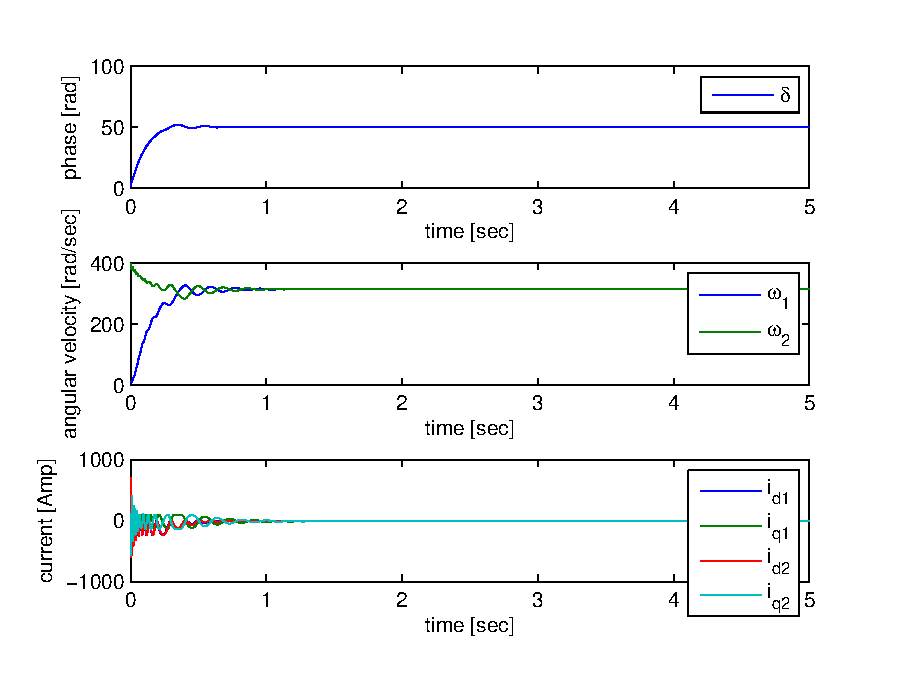
\includegraphics[scale=0.65]{5KWTICSGSimulation} \vspace{-8mm}
\caption{Simulations for TICSG system with 5KW SGs} 
\label{fig:5KWSGTICSGSimulation}
\end{figure}
%%%%%%%%%%**********%%%%%%%%%%**********%%%%%%%%%%**********%%%%%%%%%%

Figure \ref{fig:InROATICSGSimulation} shows a simulation of a TICSG 
system similar to the previous one, but with smaller $L_s$, namely
$L_s=0.41$ {[}$mH${]} (the other parameters are the same). The
initial state is close to $\Emscr$, $\left[z_1(0)\ z_2(0)\ \delta(0)
\right]^\top=\left[40,\ -20,\ 70,\ 400,\ -20,\ 65,\ 0\right]^\top$, 
such that the system stabilizes (in particular, the SGs synchronize). 

Figure \ref{fig:OutROATICSGSimulation} shows another simulation for
the same system, with the initial state $\left[z_1(0)\ z_2(0) \
\delta(0) \right]^\top=\left[-400,\ -200,\right.$ $\left. 10,\ 700,\ 
-20,\ 400,\ 1.5708\right]^\top$. \m The simu\-lation indicates that 
this initial state is outside the region of attraction, the SGs do not
synchronize.

%%%%%%%%%%**********%%%%%%%%%%**********%%%%%%%%%%**********%%%%%%%%%%
\begin{figure}[ht] % Figure 4 
\vspace{-2mm}
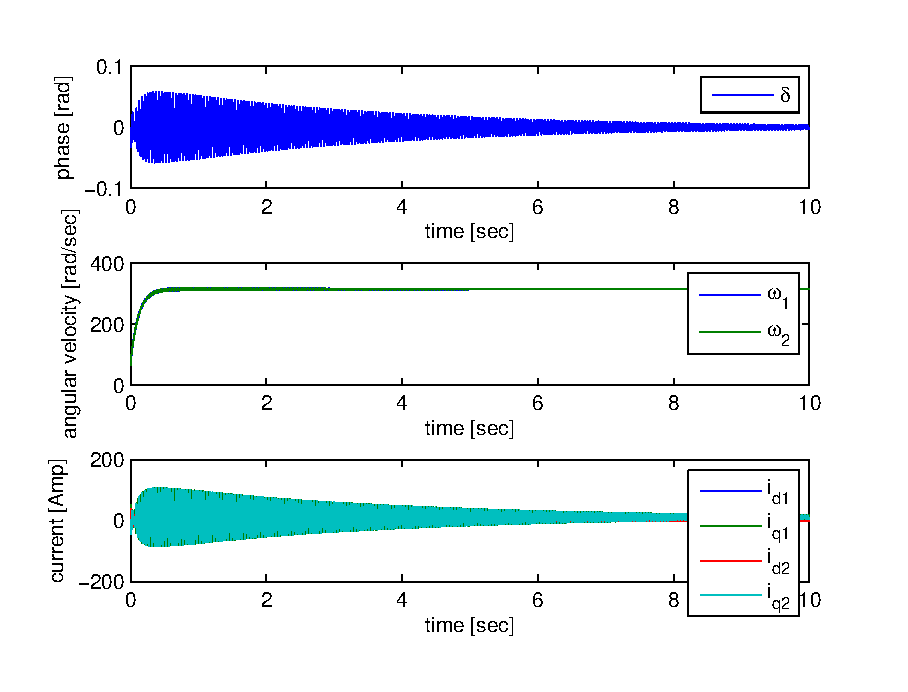
\includegraphics[scale=0.65]{InROATICSGSimulation} \vspace{-8mm}
\caption{Simulation for a TICSG system that satisfies the conditions
at the end of Section \ref{sec6}, with initial state inside the 
region of attraction of the stable equilibrium point.}
\label{fig:InROATICSGSimulation}
\end{figure}
%%%%%%%%%%**********%%%%%%%%%%**********%%%%%%%%%%**********%%%%%%%%%%

\vspace{-2mm}
%%%%%%%%%%**********%%%%%%%%%%**********%%%%%%%%%%**********%%%%%%%%%%
\begin{figure}[ht] % Figure 5
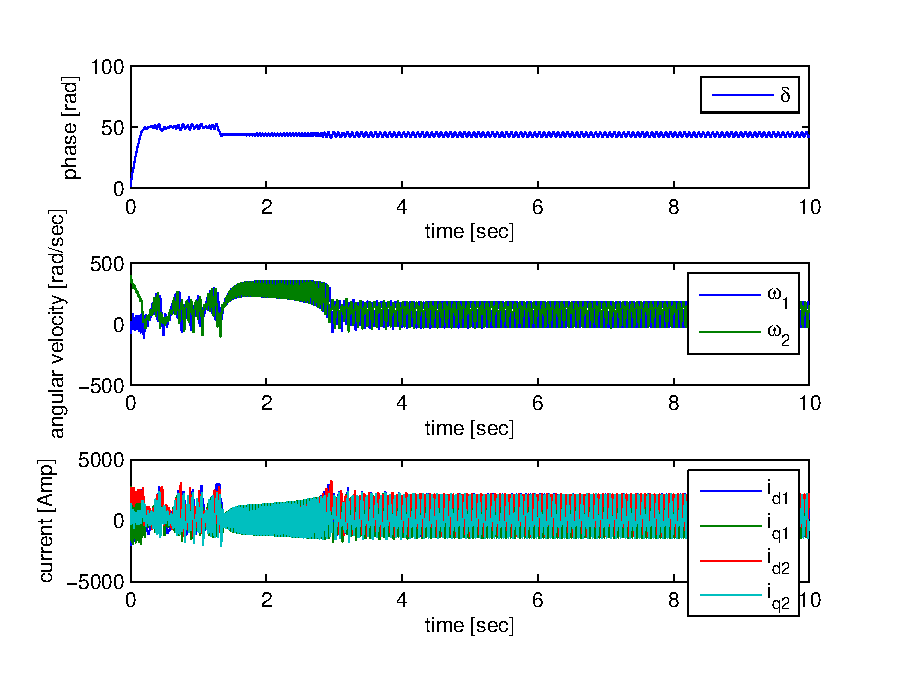
\includegraphics[scale=0.65]{OutROATICSGSimulation} \vspace{-6mm}
\caption{Simulation for a TICSG system which satisfy the conditions at
the end of Section \ref{sec6}, with initial state outside the region
of attraction of the stable equilibrium point.}
\label{fig:OutROATICSGSimulation}
\end{figure}
%%%%%%%%%%**********%%%%%%%%%%**********%%%%%%%%%%**********%%%%%%%%%%

%%%%%%%%%%++++++++++%%%%%%%%%%++++++++++%%%%%%%%%%++++++++++%%%%%%%%%%
\begin{thebibliography}{99}
 
\bibitem[Brown et~al.(2014)]{BrWe:14} E.~Brown, and G.~Weiss, \m 
 Using synchronverters for power grid stabilization, {\em IEEE 
 Convention of Electrical and Electronics Engineers in Israel}, Eilat, 
 Dec. 2014.

\bibitem[Caliskan et~al.(2014)]{CaTa:14} S.Y.~Caliskan, and 
 P.~Tabuada, \m Compositional transient stability analysis of 
 multimachine power networks, {\em IEEE Trans. Control of Network
 Syst.}, vol.~1, 2014, pp.~4-14.

\bibitem[D{\"o}rfler at~al.(2012)]{DoBull:12} F. D{\"o}rfler, and 
 F. Bullo, \m Synchronization and transient stability in power 
 networks and nonuniform Kuramoto oscillators, {\em SIAM J. Control 
 and Optim.}, vol.~50, 2012, pp.~1616-1642.

\bibitem[Fitzgerald et~al.(2003)]{Fitzgerald:03} A.E.~Fitzgerald, 
 C.~Kingsley, and S.D.~Umans, \m {\em Electric Machinery}, \m 
 McGraw-Hill, New York, 2003.

\bibitem[Galaz et~al.(2003)]{GOBS:03} M.~Galaz, R.~Ortega, 
 A.S.~Bazanella, and A.M.~Stankovic, \m An energy-shaping approach 
 to the design of excitation control of synchronous generators, 
 {\em Automatica}, vol.~39, 2003, pp.~111-119.

\bibitem[Grainger et~al.(1994)]{GrSt2014} J.J.~Grainger, and 
 W.D.~Stevenson, {\em Power Systems Analysis}, \m McGraw-Hill, New 
 York, 1994.
 
\bibitem[Green et~al.(2007)]{GreenProdanovic:07} T.~Green, and 
 M.~Prodanovic, \m Control of inverter-based micro-grids, {\em 
 Electric Power Systems Research}, vol.~77, 2007, pp.~1204-1213.
 
\bibitem[Khalil(2002)]{Khalil} H.K.~Khalil, \m \emph{Nonlinear 
 Systems} (third edition), Prentice Hall, New Jersey, 2002.

\bibitem[Kundur(1994)]{Kundur} P.~Kundur, \emph{Power System 
 Stability and Control}, McGraw-Hill, New York, 1994.

\bibitem[Mandel et~al.(2015)]{MaWe:15} Y.~Mandel and G.~Weiss, \m 
 Adaptive internal model based suppression of torque ripple in 
 brushless DC motor drives, {\em Systems Science \& Control 
 Engineering}, vol.~5, 2015, pp.~162-176.

\bibitem[Monshizadeh et~al.(2016)]{DePersiSchaft:16} 
 P.~Monshizadeh, C.~De Persis, N.~Monshizadeh, and A.~van der 
 Schaft, \m Nonlinear Analysis of an improved swing equation, \m 
 subm.~2016.

\bibitem[Natarajan et~al.(2014)]{NaWe:14} V.~Natarajan, and 
 G.~Weiss, \m Almost global asymptotic stability of a constant 
 field current synchronous machine connected to an infinite bus, 
 {\em Proc. of the 53rd IEEE Conf. on Decision and Control}, Los 
 Angeles, CA, Dec. 2014, pp.~3272-3279.

\bibitem[Natarajan et~al.(2015)]{NaWe:15} V.~Natarajan, and 
 G.~Weiss, \m Almost global asymptotic stability of a 
 grid-connected synchronous generator, submitted in 2015.

\bibitem[Sauer et~al.(1997)]{SauerPai1998} P.~W.~Sauer, and 
 M.~A.~Pai, \m {\em Power Systems Dynamics and Stability}, 
 Stipes Publishing, Champaign, IL, 1997.
  
\bibitem[Shafiee et~al.(2016)]{Shafiee_2016} Q.~Shafiee, 
 V.~Nasirian, J.C.~Vasquez, J.M.~Guerrero, and A.~Davoudi. \m 
 A multi-functional fully distributed control framework for AC 
 microgrids, {\em IEEE Trans. on Smart Grid}, to appear in 2016.

\bibitem[Schiffer et~al.(2016)]{Schiffer_2016_survey} J.~Schiffer, 
 D.~Zonetti, R.~Ortega, A.~Stankovi{\'c}, T.~Sezi, and J.~Raisch, 
 \m A survey on modeling of microgrids - from fundamental physics to
 phasors and voltage sources, {\em Automatica}, vol.~74, 2016, pp.~135-150.

\bibitem[Simpson-Porco et~al.(2013)]{PoDoBu:13} J.W.~Simpson-Porco,
 F.~D{\"o}rfler, and F.~Bullo, \m Synchronization and power sharing 
 for droop-controlled inverters in islanded microgrids, 
 {\em Automatica}, vol.~49, 2013, pp.~2603-2611.

\bibitem[Venezian et~al.(2016)]{VeWe:16} E.~Venezian, and G.~Weiss,
 \m A warning about the use of reduced models of synchronous 
 generators, \m {\em Int. Conf. on the Science of Electrical 
 Engineering} (ICSEE), Eilat, November 2016.

\bibitem[Walker(1981)]{Walker:94} J.H.~Walker, \m {\em Large 
 Synchronous Machines: Design, Manufacture and Operation}, \m Oxford 
 University Press, Oxford, 1981.

\bibitem[Zhong(2013)]{Zhong:13} Q.-C.~Zhong, \m Robust droop 
 controller for accurate proportional load sharing among inverters 
 operated in parallel, {\em IEEE Trans. on Industrial Electronics}, 
 vol.~60, 2013, pp.~1281-1290.

\bibitem[Zhong et~al.(2011)]{ZhWe:11} Q.-C.~Zhong, and G.~Weiss, \m 
 Synchronverters: Inverters that mimic synchronous generators, {\em 
 IEEE Trans. Industr. Electronics}, vol.~58, 2011, pp.~1259-1267.

\end{thebibliography}
\end{document}
